\documentclass[11pt]{article}
\usepackage[spanish]{babel}
\usepackage[utf8]{inputenc}
\usepackage[T1]{fontenc}
\usepackage{graphicx}
\topmargin=-1.2cm
\textheight=22cm
\textwidth=16cm  
\oddsidemargin=0.45cm  
\setlength{\parindent}{0cm}
\renewcommand{\baselinestretch}{1.1}
\graphicspath{{hola/}}
\title{Actividad 8}
\author{Hinostroza Moya Natalia}
\date{10 de abril de 2017}

\begin{document}
%===============================================================================
% PORTADA
%===============================================================================
\begin{titlepage}
\begin{center}
\includegraphics[scale=0.35]{escudo.png}
\end{center}
\vspace*{0.02in}
\begin{center}

\rmfamily\textbf{\LARGE UNIVERSIDAD DE SONORA}\\
\vspace*{1.02in}
{\Large División de Ciencias Exactas y Naturales}\\
{\Large Departamento de Física}\\

\vspace*{0.99in}
\rule{99mm}{0.1mm}\\
\vspace*{0.05cm}
\textbf{\LARGE Atractores Extraños\\ 
\vspace*{0.2cm}
El Efecto Mariposa}\\
\vspace*{0.001in}
\rule{99mm}{0.1mm}

\vspace*{1in}
\normalsize{Autor:}\
\normalsize{Natalia Hinostroza Moya}\\
\vspace*{0.3mm}
\normalsize Profesor:\
\normalsize Carlos Lizárraga Celaya\\
\vspace*{1.5cm}
\normalsize 18 de abril de 2017

\end{center}
\end{titlepage}

%==============================================================================
% DESARROLLO
%==============================================================================
\textbf{\section*{\LARGE Resumen}}

En el siguiente reporte se presenta una síntesis hacerca de como Edward Lorenz, estaba tratando de resolver y cómo esto llevo a toda una nueva teoría del caos. También una gráfica del atractor de Lorenz y el cómo se realizó una gráfica en movimiento para representar una partícula en el atractor de Lorenz.

\textbf{\section{\LARGE Introducción}}
Muchas veces se habla del caos de manera confusa. La palabra caos la asociamos normalmente con el desorden, descontrol, aleatoriedad, entre otras cosas parecidas. Algo impredecible e incontrolable. Pero ciertamente no es así; al menos no estrictamente. La teoría del caos tiene más cosas en común con el Efecto Mariposa que con la arbitrariedad. 

\textbf{\section{\LARGE La Teoría de Caos y Efecto Maripos}}
El "caos" es una teoría interdisciplinaria que indica que dentro de la aparente aleatoriedad de los sistemas complejos caóticos, hay patrones subyacentes, bucles de retroalimentación constantes, repetición, auto-similitud, fractales, autoorganización y confianza en la programación en el punto inicial conocido como sensible Dependencia de las condiciones iniciales.\\

En 1963, Edward Lorenz, estudió la convección en la atmósfera de la Tierra. Como las ecuaciones de Navier-Stokes que describen la dinámica de fluidos son muy difíciles de resolver, las simplifico drásticamente. El modelo probablemente tiene algo que ver con lo que realmente sucede en la atmósfera. Es un modelo de juguete, pero Lorenz pronto se dio cuenta de que es muy interesante en un sentido matemático. Si tomamos un gran número de condiciones iniciales diferentes, entonces al cabo de un tiempo todos aterrizan en el mismo objeto en forma de mariposa: el atractor de Lorenz.\\

El efecto mariposa describe cómo un pequeño cambio en un estado de un sistema no determinista puede dar lugar a grandes diferencias en un estado posterior, p. Una mariposa batiendo sus alas en Brasil puede causar un tornado en Texas.\\

La teoría del caos es una rama de las matemáticas centrada en el comportamiento de los sistemas dinámicos que son altamente sensibles a las condiciones iniciales.\\

El comportamiento caótico existe en muchos sistemas naturales, como el clima y el tiempo. También ocurre espontáneamente en algunos sistemas con componentes artificiales, como el tráfico por carretera. Este comportamiento puede ser estudiado a través del análisis de un modelo matemático caótico, o a través de técnicas analíticas tales como parcelas de repetición y mapas de Poincaré.\\

La teoría del caos tiene aplicaciones en varias disciplinas, incluyendo la meteorología, la sociología, la física, la ciencia ambiental, la informática, la ingeniería, la economía, la biología, la ecología y la filosofía. La teoría formó la base para tales campos de estudio como los sistemas dinámicos complejos, el borde de la teoría del caos, el proceso de autoensamblaje.

\textbf{\section{\LARGE Resultado de los gráficos realizados en Phyton}}

El código para gráficar el Atractor de Lorenz que se utilizó es el siguiente:\\

\begin{verbatim}
def lorenz(x, y, z, s=10, r=28, b=2.667):
    x_dot = s*(y - x)
    y_dot = r*x - y - x*z
    z_dot = x*y - b*z
    return x_dot, y_dot, z_dot

dt = 0.01
stepCnt = 10000

s = np.empty((stepCnt + 1,))
ys = np.empty((stepCnt + 1,))
zs = np.empty((stepCnt + 1,))

xs[0], ys[0], zs[0] = (0., 1., 1.05)

for i in range(stepCnt):
    # Derivatives of the X, Y, Z state
    x_dot, y_dot, z_dot = lorenz(xs[i], ys[i], zs[i])
    xs[i + 1] = xs[i] + (x_dot * dt)
    ys[i + 1] = ys[i] + (y_dot * dt)
    zs[i + 1] = zs[i] + (z_dot * dt)
    
fig = plt.figure()
ax = fig.gca(projection='3d')

ax.plot(xs, ys, zs, lw=0.3)
ax.set_xlabel("X Axis")
ax.set_ylabel("Y Axis")
ax.set_zlabel("Z Axis")
ax.set_title("Atractor de Lorenz")

plt.show()
\end{verbatim}

Se obtuvo lo siguiente.\\

\begin{center}
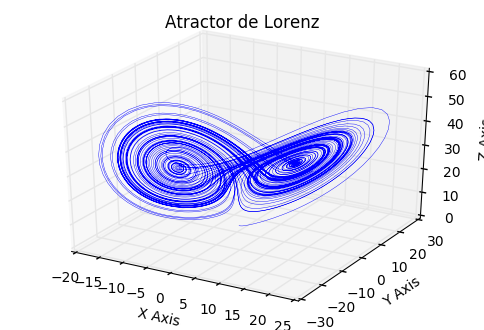
\includegraphics[]{AL.png}
\end{center}

\vspace*{1cm}

Con una animación creada en Python de una partícula que tenía un movimiento repetitivo pude notar mucho mejor lo que decia Lorenz sobre que la partícula volvería a estar de nuevo en el mismo lugar en un cierto tiempo creando así una gráfica en forma de mariposa, que es la que observamos arriba. 

\end{document}
